\documentclass{beamer}

\usetheme{Madrid}

\usepackage[orientation=portrait,size=a1,scale=1]{beamerposter}
\usepackage[overlay]{textpos}

\usepackage[utf8]{inputenc}
\usepackage{default}
\usepackage{changepage}
\usepackage{subfigure}
\usepackage[labelformat=empty]{caption}

\setlength{\columnsep}{5cm}

\usepackage{tikz}
\usetikzlibrary{calc}
\tikzset{egrid/.style={draw,help lines}}
\tikzset{mgrid/.style={draw,help lines,dashed}}
\tikzset{epoint/.style={draw,circle,red,inner sep=2pt,fill}}
\tikzset{mpoint/.style={draw,circle,blue,inner sep=2pt,fill}}

\definecolor{dark}{RGB}{0,105,0}

\setbeamertemplate{background canvas}[vertical shading][top=yellow!80!dark,bottom=yellow!60!dark]
\beamertemplatenavigationsymbolsempty
\setbeamertemplate{blocks}[rounded][shadow=false]
\setbeamercolor{block body}{bg=yellow!30}
\setbeamercolor{block title}{bg=dark}
\setbeamercolor{item}{fg=dark}

\title{Modeling of light propagation through smectic waveguides}

\author{\underline{Miha \v Can\v cula\inst{1}}\and Miha Ravnik\inst{1}\and Slobodan \v Zumer\inst{1,2}}
\institute{\inst{1}Faculty of Mathematics and Physics, University of Ljubljana\and\inst{2}Jo\v zef Stefan Institute, Ljubljana}

\newcommand{\blockpadding}{
  \rule[-0.6ex]{0pt}{2.5ex}
}

\addtobeamertemplate{block begin}
  {\vspace{1ex}}
  {\vspace{1ex} % Pads top of block
     % separates paragraphs in a block
   \setlength{\parskip}{24pt plus 1pt minus 1pt}%
   \begin{adjustwidth}{1cm}{1cm}
}
\addtobeamertemplate{block end}
  {\end{adjustwidth}%
   \vspace{1ex}}% Pads bottom of block
  {} % Seperates blocks from each other

\begin{document}

\begin{columns}
 \begin{column}{.976\textwidth}
  \begin{block}{}
\vspace{0.5cm}
\centering
{\Huge \inserttitle} \\
\vspace{1cm}
{\LARGE \insertauthor} \\
\vspace{1cm}
\insertinstitute
\vspace{0.5cm}
\end{block}


 \end{column}
\end{columns}
\begin{columns}[t]
 \begin{column}{.36\textwidth}
\begin{block}{\blockpadding Motivation}
\begin{itemize}
  \setlength{\itemsep}{20pt}
 \item Light guiding structure play an important role in modern communication systems
 \item Unique optical properties of liquid crystals make them extremely useful for guiding light
 \item Smectic fibres with radial director can be created in a laboratory using 8CB and a surfactant\cite{musevic-nekej}
 \item Point defect in a nematic droplet turns a Gaussian beam into Laguerre-Gaussian -- is there a similar effect caused by the line defect in a fibre?
\end{itemize}
\end{block}

\begin{block}{\blockpadding Methods}
 \begin{itemize}
   \setlength{\itemsep}{20pt}
  \item FDTD method in 3D with anisotropic $\varepsilon$
  \item PBC in $z$ direction -- infinite cylindrical waveguide
  \item Observe propagation of Gaussian laser pulse
  \item Staggered grid, adapted for dielectric anisotropy
 \begin{figure}[h]
\centering
 \subfigure{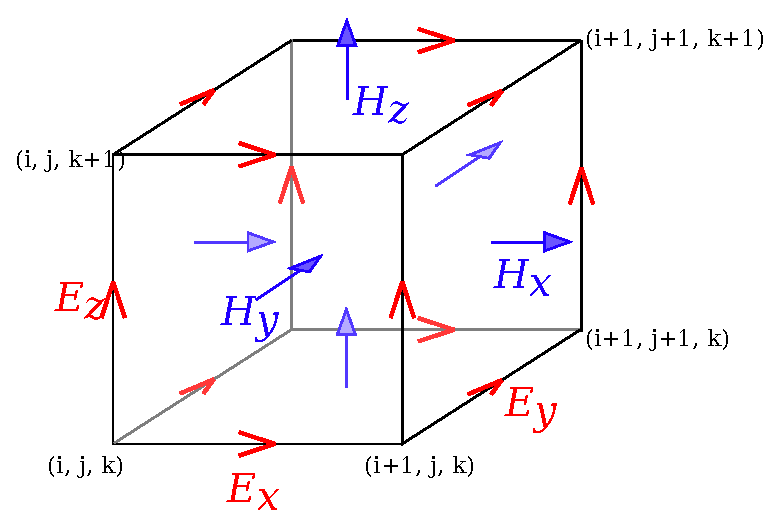
\includegraphics[width=.4\textwidth]{../Magisterij/Slike/Yee-cube}}
 \subfigure{\begin{tikzpicture}[scale=1.4]
    
    \foreach \x in {0,1}{
      \foreach \y in {0,1}{
        \node[mpoint] at (2*\x,2*\y) {}; 
        \node[mpoint] at (2*\x+1.2,2*\y+0.8) {}; 
        \node[epoint] at (2*\x+1.6,2*\y+1.4) {};
        \node[epoint] at (2*\x+1.6-1.2,2*\y+1.4-0.8) {};
        \draw[mgrid] (2*\x,2*\y) -- (2*\x+1.2,2*\y+0.8);
        \draw[egrid] (2*\x+1.6,2*\y+1.4) -- (2*\x+1.6-1.2,2*\y+1.4-0.8);
      }
    }
    
    \draw[mgrid] (0,0) rectangle (2,2);
    \draw[mgrid] (1.2,0.8) rectangle (3.2,2.8);
    \draw[egrid] (1.6,1.4) rectangle (3.6,3.4);
    \draw[egrid] (1.6-1.2,1.4-0.8) rectangle (3.6-1.2,3.4-0.8);
\end{tikzpicture}}
\label{fig:lattice}
\caption{{\color{dark} Left:} Yee lattice, optimized for diagonal dielectric tensor. \\{\color{dark} Right:} The lattice we used, suitable for full anisotropic $\varepsilon$. \\In both cases $\vec E$ and $\vec H$ are known at different times}
\end{figure}

\item Cylindrical waveguide with a radial director profile and a singular disclination line along its axis \\
\begin{figure}[h]
\centering
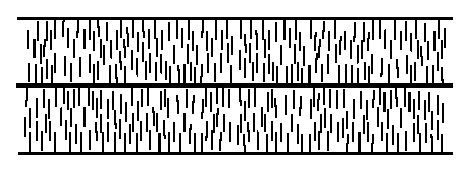
\includegraphics[width=.5\textwidth]{../Magisterij/Slike/director-profile-radial}
\end{figure}

 \end{itemize}
 \end{block}

 \end{column}
 
 \begin{column}{0.596\textwidth}
  \begin{block}{\blockpadding Results}
We showed that a Gaussian beam entering a fibre quickly turns into a Laguerre-Gaussian beam, and then into something else. 
\end{block}
 \end{column}

\end{columns}

\begin{textblock}{5.5}(0.5,5.75)
 

\end{textblock}

\begin{textblock}{8.5}(6.5,2.5)

\end{textblock}

\end{document}
